\documentclass[10,twocolumn]{article}
\usepackage[utf8]{inputenc}
%\usepackage{hyperref}

\title{QuickCHecking C kod i Haskell}
\author{Sebastian Lagerman \\ seblag@student.chalmers.se}
%\author{Sebastian Lagerman \\ \href{mailto:seblag@student.chalmers.se}{seblag@student.chalmers.se}}
\date{October 2016}

\usepackage{natbib}
\usepackage{graphicx}

\begin{document}

\maketitle

Backgrounds:

Intro. FP, Datastructures, C, AFP

\section{Introduction}
% Briefly describe and motivate the project, and convince the reader of the importance of the proposed thesis work.
% A good introduction will answer these questions:
% Why is addressing these challenges significant for gaining new knowledge in the studied domain?
% How and where can this new knowledge be applied?

Testing of code is important and a way of testing code is to generate tests and testing properties.
A useful property based testing tool is QuickCheck however currently it cannot check C libraries without other modules. % Maybe reference?
An interesting problem could then be to streamline the process of testing C code in the QuickCheck module in Haskell.
% An interesting extension to QuickCheck could then be to parse a C library and generate the boiler plate code for testing the library with the QuickCheck module in Haskell.



% build a tool to parse C files to construct the boiler plate code for the module inline-c.

% The goal of this proposal is to build a tool or application that one can use to QuickCheck C code against a Haskell specification.
% Then use this to test open-source libraries in C, for example for data structures, image manipulation, compression, encryption, etc.
% This tool will be a good way to streamline the testing to ensure software quality.
% Knowledge of this will hopefully be useful in code testing to reduce the amount of time spent on writing tests for code.
% For this Master thesis it will be tested on open source C code.
% \ref{QuickCheckAUTOSAR}



\section{Context}

% Use one or two high quality references for providing evidence from the literature that the proposed study indeed includes scientific and engineering challenges, or is related to existing ones.
% Convince the reader that the problem addressed in this thesis has not been solved prior to this project.

Prior work has already been done towards QuickChecking libraries in Erlang \citep{QuickCheckAUTOSAR}.
However, this particular tool utilises Erlang instead of Haskell and isn't an open-source project.
% non commerce use?

Similarly there exists property based testing libraries in C \citep{theft}.
This leaves us with a very interesting options, to extend Haskells QuickChecking to be able to test C libraries.


\section{Goals and Challenges}

% Describe your contribution with respect to concepts, theory and technical goals.
% Ensure that the scientific and engineering challenges stand out so that the reader can easily recognise that you are planning to solve an advanced problem.

The goal of the project is to create a tool for generating boiler plate code for tests for C libraries.
The tool should be easy to use for a developer with knowledge in both C and Haskell development.

% Another way to solve this problem would be to create and use a property-based library in C, however this has already been done by Scott Vokes \citep{theft}.
% To avoid reinventing the wheel and to improve Chalmers own QuickCheck we propose to use Haskell instead.
% This would make the goal to provide a Haskell module for QuickChecking properties for the following C libraries:
The module can be tested on the following open source libraries to begin with to later move on to harder libraries with structs.

\begin{itemize}
  % \item limits
  \item cmath
  \item string
  \item time
  % \item uchar
  % \item wchar
  % \item wctype
\end{itemize}

These were chosen because they are commonly used libraries in C development \citep{website:en.wikipedia.org} which also only uses primitive types in C.
% It will be good to use some standard libraries to start with to make sure that the problems that are found in the beginning actually occur inside the testing module that will be created.
More libraries may be added if time permits. % such as a library that contains bugs.

Some possible libraries that could be created with structs in them for testing the generation of types, could be:

\begin{itemize}
  % \item data structures
  % \item image manipulation
  \item compression
  \item encryption
\end{itemize}

The module will be tested and verified with QuickCheck though the properties will be found during development.


\section{Approach}

Various scientific approaches are appropriate for different challenges and project goals.
Outline and justify the ones that you have selected.
For example, when your project considers systematic data collection, you need to explain how you will analyze the data, in order to address your challenges and project goals.

One scientific approach is to use formal models and rigorous mathematical argumentation to address aspects like correctness and efficiency.
If this is relevant, describe the related algorithmic subjects, and how you plan to address the studied problem.
For example, if your plan is to study the problem from a computability aspect, address the relevant issues, such as algorithm and data structure design, complexity analysis, etc.
If you plan to develop and evaluate the prototype, briefly describe your plans to design, implement, and evaluate your prototype by reviewing at most two relevant issues, such as key functionalities and their evaluation criteria.{Approach}

Various scientific approaches are appropriate for different challenges and project goals.
Outline and justify the ones that you have selected.
For example, when your project considers systematic data collection, you need to explain how you will analyze the data, in order to address your challenges and project goals.

One scientific approach is to use formal models and rigorous mathematical argumentation to address aspects like correctness and efficiency.
If this is relevant, describe the related algorithmic subjects, and how you plan to address the studied problem.
For example, if your plan is to study the problem from a computability aspect, address the relevant issues, such as algorithm and data structure design, complexity analysis, etc.
If you plan to develop and evaluate the prototype, briefly describe your plans to design, implement, and evaluate your prototype by reviewing at most two relevant issues, such as key functionalities and their evaluation criteria.{Approach}

Various scientific approaches are appropriate for different challenges and project goals.
Outline and justify the ones that you have selected.
For example, when your project considers systematic data collection, you need to explain how you will analyze the data, in order to address your challenges and project goals.

One scientific approach is to use formal models and rigorous mathematical argumentation to address aspects like correctness and efficiency.
If this is relevant, describe the related algorithmic subjects, and how you plan to address the studied problem.
For example, if your plan is to study the problem from a computability aspect, address the relevant issues, such as algorithm and data structure design, complexity analysis, etc.
If you plan to develop and evaluate the prototype, briefly describe your plans to design, implement, and evaluate your prototype by reviewing at most two relevant issues, such as key functionalities and their evaluation criteria.{Approach}

Various scientific approaches are appropriate for different challenges and project goals.
Outline and justify the ones that you have selected.
For example, when your project considers systematic data collection, you need to explain how you will analyze the data, in order to address your challenges and project goals.

One scientific approach is to use formal models and rigorous mathematical argumentation to address aspects like correctness and efficiency.
If this is relevant, describe the related algorithmic subjects, and how you plan to address the studied problem.
For example, if your plan is to study the problem from a computability aspect, address the relevant issues, such as algorithm and data structure design, complexity analysis, etc.
If you plan to develop and evaluate the prototype, briefly describe your plans to design, implement, and evaluate your prototype by reviewing at most two relevant issues, such as key functionalities and their evaluation criteria.{Approach}

Various scientific approaches are appropriate for different challenges and project goals.
Outline and justify the ones that you have selected.
For example, when your project considers systematic data collection, you need to explain how you will analyze the data, in order to address your challenges and project goals.

One scientific approach is to use formal models and rigorous mathematical argumentation to address aspects like correctness and efficiency.
If this is relevant, describe the related algorithmic subjects, and how you plan to address the studied problem.
For example, if your plan is to study the problem from a computability aspect, address the relevant issues, such as algorithm and data structure design, complexity analysis, etc.
If you plan to develop and evaluate the prototype, briefly describe your plans to design, implement, and evaluate your prototype by reviewing at most two relevant issues, such as key functionalities and their evaluation criteria.{Approach}

Various scientific approaches are appropriate for different challenges and project goals.
Outline and justify the ones that you have selected.
For example, when your project considers systematic data collection, you need to explain how you will analyze the data, in order to address your challenges and project goals.

One scientific approach is to use formal models and rigorous mathematical argumentation to address aspects like correctness and efficiency.
If this is relevant, describe the related algorithmic subjects, and how you plan to address the studied problem.
For example, if your plan is to study the problem from a computability aspect, address the relevant issues, such as algorithm and data structure design, complexity analysis, etc.
If you plan to develop and evaluate the prototype, briefly describe your plans to design, implement, and evaluate your prototype by reviewing at most two relevant issues, such as key functionalities and their evaluation criteria.

\begin{itemize}
  \item The design and implementation should specify prototype properties, such as functionalities and performance goals, e.g., scalability, memory, energy.
    Motivate key design, with respect to state of the art and existing platforms, libraries, etc.
  \item When discussing evaluation criteria, describe the testing environment, e.g., test-bed experiments, simulation, and user studies, which you plan to use when assessing your prototype.
    Specify key tools, and preliminary test-case scenarios.
    Explain how and why you plan to use the evaluation criteria in order to demonstrate the functionalities and design goals.
    Explain how you plan to compare your prototype to the state of the art using the proposed test-case evaluation scenarios and benchmarks.
\end{itemize}


\section{References}

Reference all sources that are cited in your proposal using, e.g.\ the APA, Harvard$^{2}$, or IEEE$^{3}$ style


%\section{Introduction}
%There is a theory which states that if ever anyone discovers exactly what the Universe is for and why it is here, it will instantly disappear and be replaced by something even more bizarre and inexplicable.
%There is another theory which states that this has already happened.
%\section{Introduction}
% Briefly describe and motivate the project, and convince the reader of the importance of the proposed thesis work.
% A good introduction will answer these questions:
% Why is addressing these challenges significant for gaining new knowledge in the studied domain?
% How and where can this new knowledge be applied?

Testing of code is important and a way of testing code is to generate tests and testing properties.
A useful property based testing tool is QuickCheck however currently it cannot check C libraries without other modules. % Maybe reference?
An interesting problem could then be to streamline the process of testing C code in the QuickCheck module in Haskell.
% An interesting extension to QuickCheck could then be to parse a C library and generate the boiler plate code for testing the library with the QuickCheck module in Haskell.



% build a tool to parse C files to construct the boiler plate code for the module inline-c.

% The goal of this proposal is to build a tool or application that one can use to QuickCheck C code against a Haskell specification.
% Then use this to test open-source libraries in C, for example for data structures, image manipulation, compression, encryption, etc.
% This tool will be a good way to streamline the testing to ensure software quality.
% Knowledge of this will hopefully be useful in code testing to reduce the amount of time spent on writing tests for code.
% For this Master thesis it will be tested on open source C code.
% \ref{QuickCheckAUTOSAR}



%\begin{figure}[h!]
%\centering
%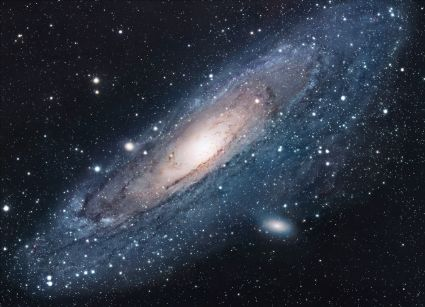
\includegraphics[scale=1.7]{universe.jpg}
%\caption{The Universe}
%\label{fig:univerise}
%\end{figure}

%\section{Conclusion}
%``I always thought something was fundamentally wrong with the universe'' \citep{adams1995hitchhiker}

%\bibliographystyle{plain}
%\bibliography{references}

\end{document}
